\documentclass[10pt,a4paper]{article}
\usepackage[english]{babel}
\usepackage[utf8]{inputenc}
\usepackage{amsmath}
\usepackage{amsfonts}
\usepackage{amssymb}
\usepackage{graphicx}
\usepackage{caption}
\usepackage{subcaption}
\usepackage{url}
%\usepackage{fullpage}

\DeclareMathOperator*{\argmax}{arg\,max}

\author{Joan Puigcerver Pérez\\
\footnotesize{\texttt{joapuipe@upv.es}}}
\title{Statistical Machine Translation: Part I and II}
\begin{document}
\maketitle
\section{Introduction}\label{sec:intro}
This work shows the results obtained for different exercises proposed in the course \emph{Statistical Machine Translation} (SMT). Three effects have been studied: the effect on the translation quality (BLEU) when using $k$-tuples of words as basic units instead of single words, the degradation of the original source data after multiple translation rounds and, finally, the effect on the translation quality using semi-supervised data.\\

In this work, phrase-based translation models are used. The language models (LMs) are $N$-gram models trained using SRILM toolkit. Language models use Good-Turing discounting and linear interpolation as smoothing. The other models (alignment, reordering, ...) are trained using the popular Moses toolkit (which uses GIZA++ to train the alignment models). The complete translation model is a log-linear model which weights log-probability scores obtained by different models.\\

\begin{equation}
\hat{y} = \argmax_{y \in \Sigma^+} \sum_{m=1}^M \lambda_m h_m(x, y)
\end{equation}

Each of the $h_m(x,y)$ terms is the score given by one of the models used. We used the default models used by Moses which includes 15 different models (including the word insertion penalty). These 15 weights can be optimized using a validation set and the MERT technique.\\

In order to explore the described effects, the EuTrans-I corpus\footnote{\url{https://prhlt.iti.upv.es/projects/translation/eutrans/EuTrans1BenchmarkRelease.tgz}} has been used. This dataset contains 13000 parallel sentences in Spanish and English. 10000 of those sentences are used for training and the remaining 3000 for the final test set. In order to optimize the weights of the of the translation models, 200 random samples from the training set have been extracted to form a validation set for MERT. 5-fold cross-validation is used to train all the models on the remaining 9800 phrases and optimize the LM model order and the word $k$-tuples size.\\

All the results shown in this report can be reproduced using the same scripts as the author used, which are available on the Internet\footnote{\url{https://github.com/jpuigcerver/miarfid-smt}}.

\section{Using tuples of words as basic elements}\label{sec:tuples}
Here we explore the effect of considering $k$-tuples of words instead of single words as basic translation units. For instance, the phrase ``\emph{the red cross building is close}'' could be interpreted as 2-tuples of words by ``\emph{\$\_the the\_red red\_cross cross\_building building\_is is\_close}''. We simply transformed the original data set to different sizes of $k$-tuples ($k \in \{2,3,4\}$), and then the language models and translation models were trained as usual on this transformed data. Tables \ref{tab:tuples_valid_es_en} (Spanish to English translation) and \ref{tab:tuples_valid_en_es} (English to Spanish translation) show the results of this procedure evaluated on the validation set. To compute all the BLEU scores in this region, the output of the translation model is \emph{detuplified} and compared against the original reference.\\

\begin{table}[h]
\centering
\begin{subfigure}[b]{0.9\textwidth}
\centering
\begin{tabular}{|l|c|c|c|c|}
\hline
LM & 1-tuple & 2-tuple & 3-tuple & 4-tuple\\
\hline
2-grams & $90.72 \pm 0.23$ & $87.79 \pm 0.27$ & $79.79 \pm 0.25$ & $69.12 \pm 0.65$\\
3-grams & $91.35 \pm 0.25$ & $87.91 \pm 0.40$ & $79.76 \pm 0.36$ & $68.82 \pm 0.76$\\
4-grams & $92.04 \pm 0.34$ & $\mathbf{88.43 \pm 0.29}$ & $79.67 \pm 0.60$ & $69.21 \pm 0.77$\\
5-grams & $92.13 \pm 0.57$ & $88.27 \pm 0.33$ & $79.76 \pm 0.45$ & $68.77 \pm 0.83$\\
6-grams & $\mathbf{92.22 \pm 0.36}$ & $88.17 \pm 0.38$ & $\mathbf{79.94 \pm 0.37}$ & $\mathbf{69.29 \pm 0.99}$\\
7-grams & $92.17 \pm 0.38$ & $88.21 \pm 0.35$ & $79.85 \pm 0.36$ & $68.98 \pm 1.08$\\
\hline
\end{tabular}
\caption{Spanish to English translation}
\label{tab:tuples_valid_es_en}
\end{subfigure}\\

\begin{subfigure}[b]{0.9\textwidth}
\centering
\begin{tabular}{|l|c|c|c|c|}
\hline
LM & 1-tuple & 2-tuple & 3-tuple & 4-tuple\\
\hline
2-grams & $67.25 \pm 0.63$ & $\mathbf{66.65 \pm 0.50}$ & $60.81 \pm 0.70$ & $55.16 \pm 1.07$\\
3-grams & $67.68 \pm 0.33$ & $66.47 \pm 0.23$ & $60.17 \pm 0.62$ & $55.20 \pm 0.73$\\
4-grams & $68.03 \pm 0.50$ & $66.06 \pm 0.42$ & $60.67 \pm 0.32$ & $55.75 \pm 0.59$\\
5-grams & $67.93 \pm 0.34$ & $66.45 \pm 0.59$ & $60.26 \pm 0.74$ & $55.22 \pm 0.80$\\
6-grams & $\mathbf{68.22 \pm 0.43}$ & $66.45 \pm 0.77$ & $59.83 \pm 0.42$ & $54.84 \pm 1.01$\\
7-grams & $67.85 \pm 0.23$ & $66.42 \pm 0.62$ & $\mathbf{61.52 \pm 0.37}$ & $\mathbf{56.07 \pm 1.10}$\\
\hline
\end{tabular}
\caption{English to Spanish translation}
\label{tab:tuples_valid_en_es}
\end{subfigure}
\caption{BLEU on the validation set for different configurations explored of $k$-tuples  sizes and $N$-grams sizes.}
\label{tab:tuples_valid}
\end{table}

Notice that using $k$-tuples instead of single words makes the translation accuracy worse. As the number of $k$ increases, the number of unobserved tuples will increase exponentially, as it happens with the $N$-grams language models when $N$ increases. Moreover, here no sort of backoff or interpolation for the translation models is done as it is done by Language Models to handle unobserved events, because we lost the original single words. Thus, the number of out-of-vocabulary (OOV) tuples increases with the $k$-tuples size. Figures \ref{fig:oov_dict} and \ref{fig:oov_global} show this effect on the same data than experiments from table \ref{tab:tuples_valid}. Figure \ref{fig:oov_dict} shows the OOV rate computed as $\frac{|V_{ref}| - |V_{train}|}{|V_{ref}|}$, so this one does not consider repetitions of any tuple. However, figure \ref{fig:oov_global} does count the repetitions of tuples and thus, is more indicative about how the OOV tuples affect the accuracy of the translations. It is computed as: $\frac{\sum_{w \in V_{ref} : w \notin V_{train}} Count(w, T_{ref})}{|T_{ref}|}$. Observe that the OOV running tuples go from almost 0\%, when using single words (1-tuples), to 5\% for English and 9\% for Spanish, when using 4-tuples of words. And most important, the exponential shape of the histogram.\\

\begin{figure}[h]
\centering
\begin{subfigure}[b]{0.485\textwidth}
\centering
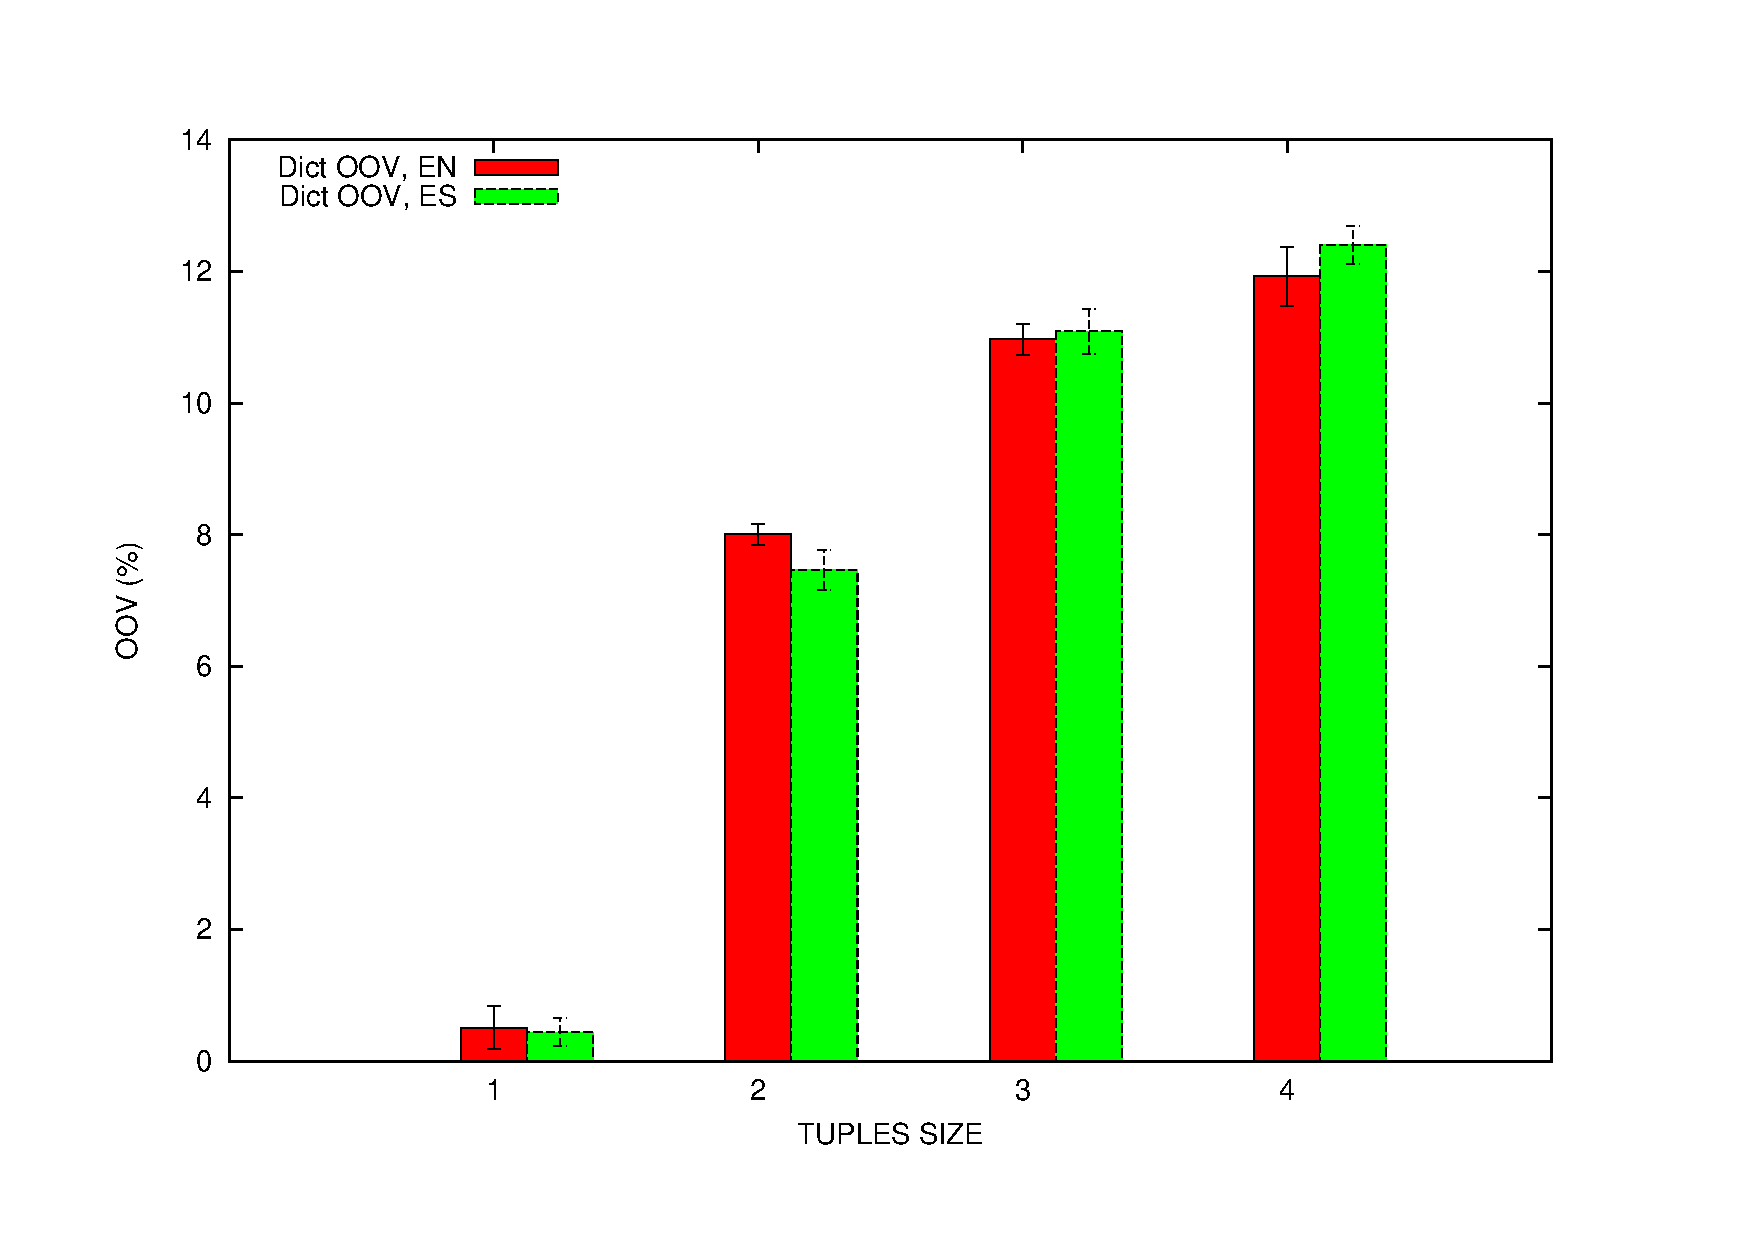
\includegraphics[width=\textwidth]{OOV_dict.pdf}
\caption{OOV tuples respect the dictionary size of the reference (this does not count repetitions).}
\label{fig:oov_dict}
\end{subfigure}
~
\begin{subfigure}[b]{0.485\textwidth}
\centering
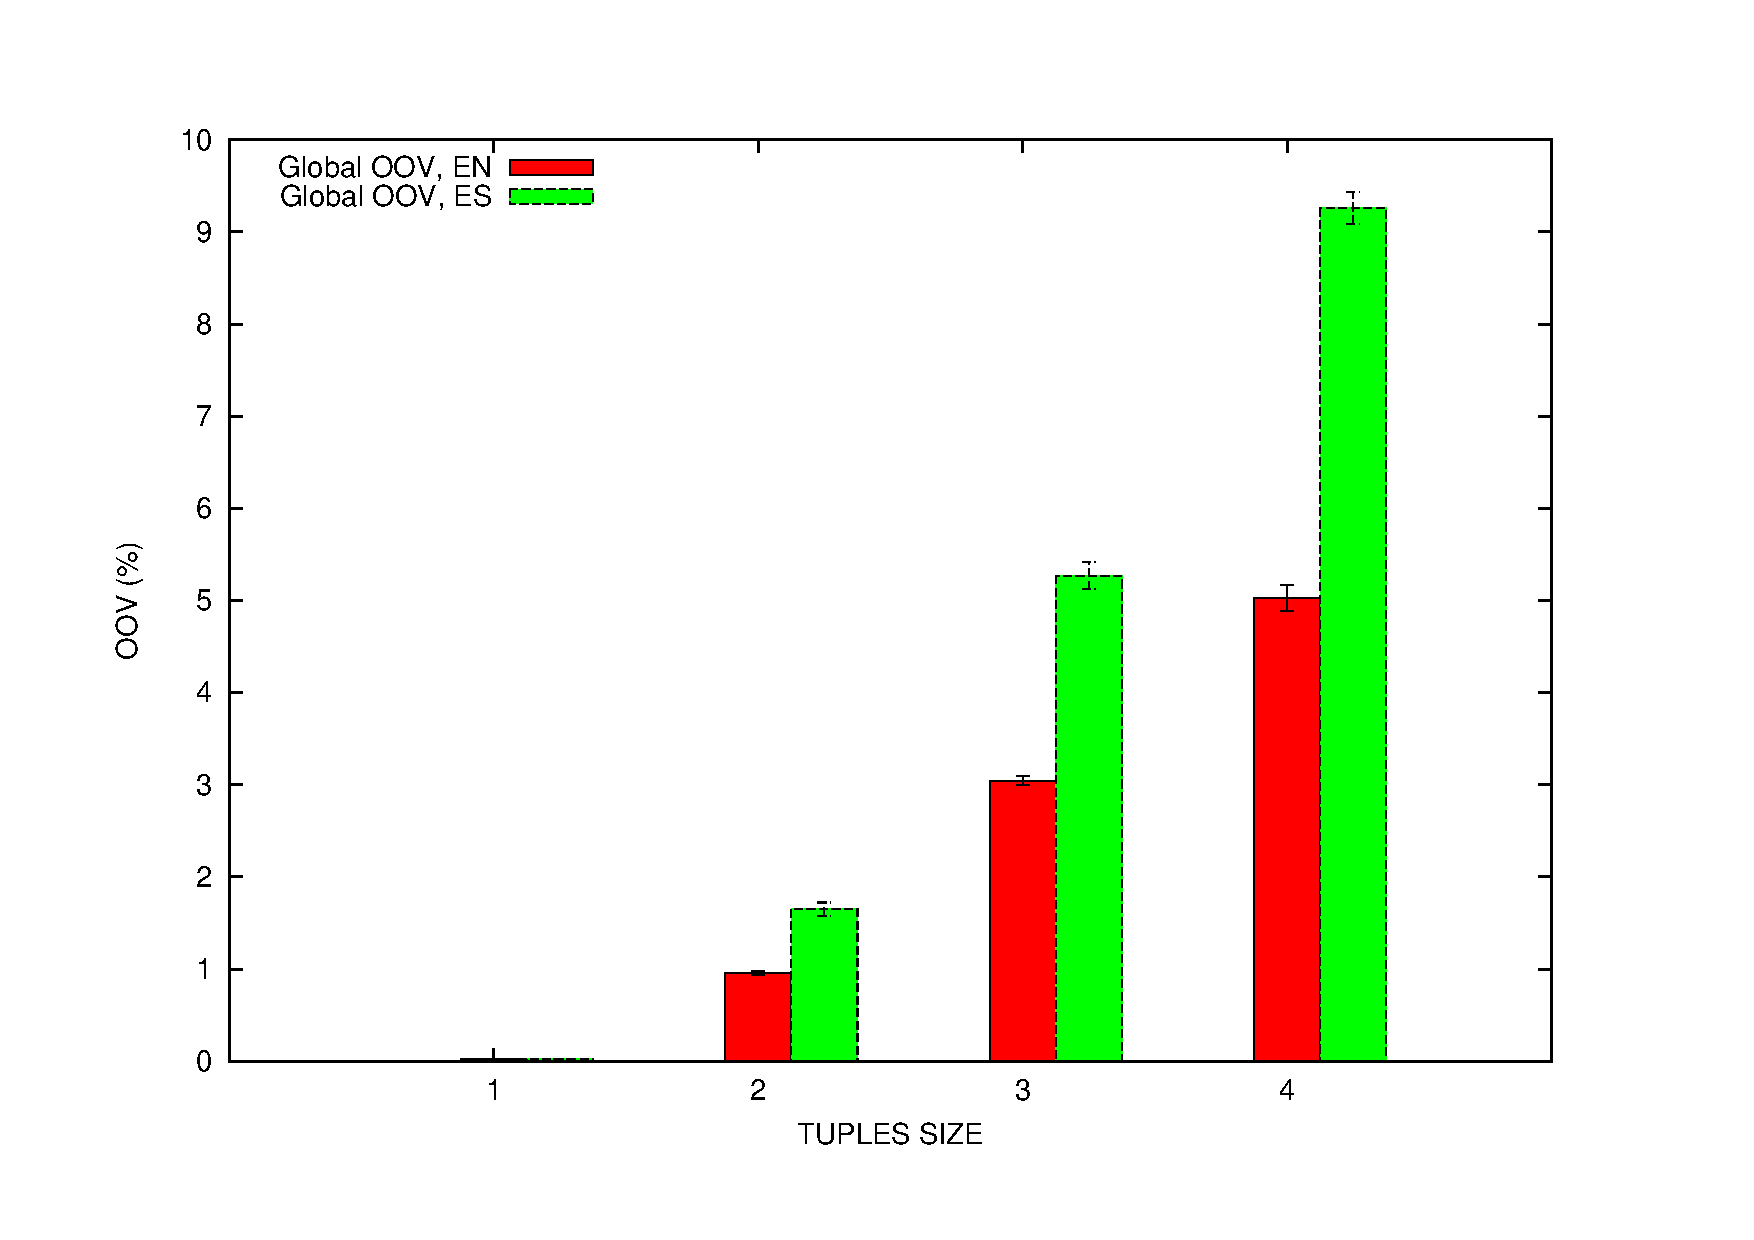
\includegraphics[width=\textwidth]{OOV_global.pdf}
\caption{OOV tuples respect the total number of words in the reference (this does count repetitions).}
\label{fig:oov_global}
\end{subfigure}
\caption{Effect on the OOV rate with the increase of the $k$-tuples size. Results obtained using 5-fold cross-validation. Confidence intervals at 95\%.}
\label{fig:oov}
\end{figure}

The effect of the language model size depends on the language, as it is shown in figure \ref{fig:monowords_ngram}. This figure shows the average BLEU with confidence intervals for different sizes of the $N$-gram language models when using single words as basic units (first column from tables \ref{tab:tuples_valid_es_en} and \ref{tab:tuples_valid_en_es}). When translating from English to Spanish, all the confidence intervals overlap for the different language model sizes tried. However, when translating from Spanish to English, $2$-grams and $3$-grams are significantly worse than the rest.\\

\begin{figure}[h]
\centering
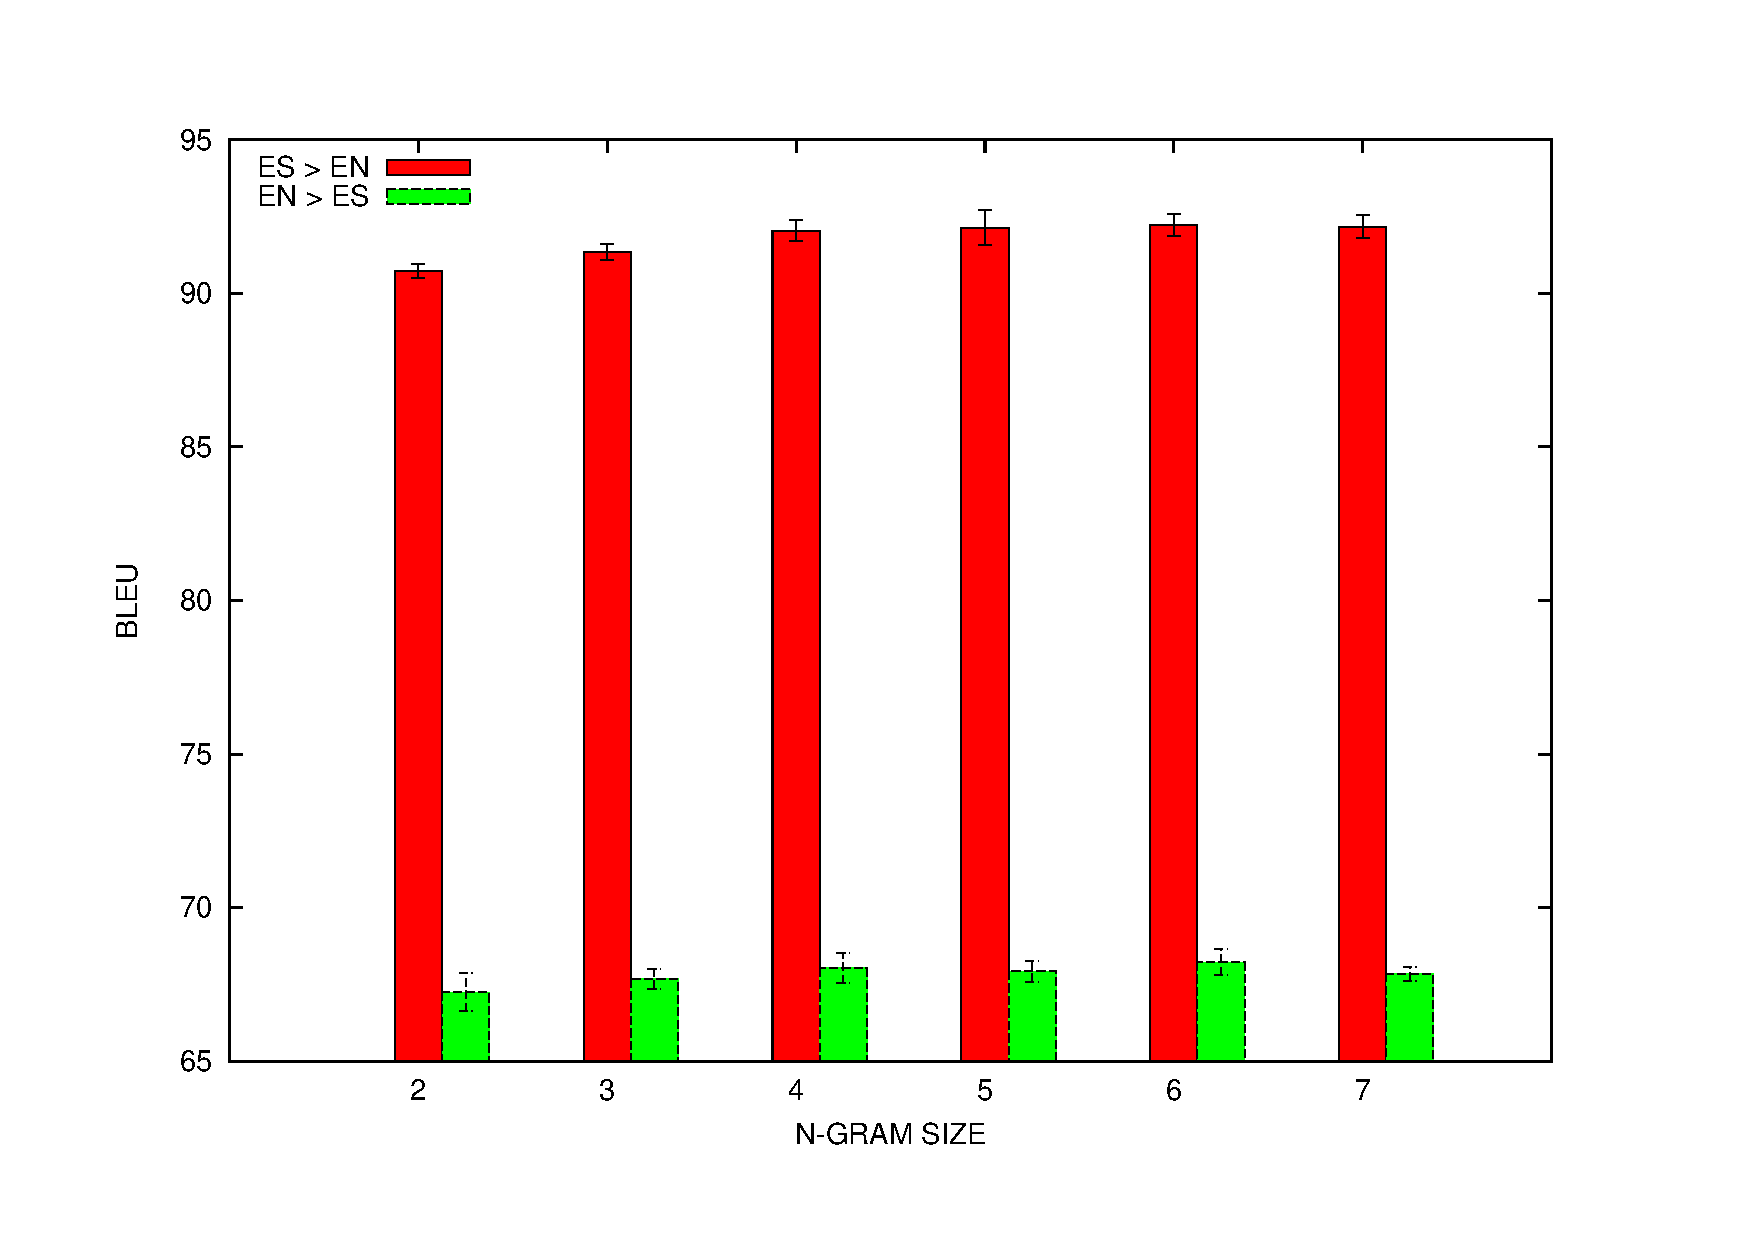
\includegraphics[width=0.7\textwidth]{monowords_ngram_size.pdf}
\caption{Effect of the $N$-gram language model size on the BLEU, using single words as basic units. Results obtained using 5-fold cross-validation. Confidence intervals at 95\%.}
\label{fig:monowords_ngram}
\end{figure}

Table \ref{tab:test} shows the performance on the test set for the different configurations of $k$-tuples. The language model used in combination of each $k$-tuple is the one which reported the highest BLEU on the validation set for the given $k$-tuple.

\begin{table}[h]
\centering
\begin{tabular}{|l|c|c|c|c|}
\hline
Direction & 1-tuple & 2-tuple & 3-tuple & 4-tuple\\
\hline
ES $\rightarrow$ EN & $\textbf{90.78} ~ (N=6)$ & $87.63 ~ (N=4)$ & $77.13 ~ (N=6)$ & $63.93 ~ (N=6)$ \\
EN $\rightarrow$ ES & $\textbf{67.95} ~ (N=6)$ & $65.89 ~ (N=2)$ & $58.13 ~ (N=7)$ & $52.18 ~ (N=7)$ \\
\hline
\end{tabular}
\caption{BLEU on the test set for different $k$-tuples sizes. The language model size is indicated by the variable $N$.}
\label{tab:test}
\end{table}

\section{Degradation effect after iterative translation}
This work shows the degradation effect of iteratively translating the source text to a target language, and the translating back from the target language to the original source language (this is what we will refer as one ``round''). The degradation is measured using the BLEU score between the original source file, and the file produced after several rounds of the described procedure. Observe that, when the number of translation rounds is zero, the BLEU is 100, since the reference text is compared against itself.\\

In order to run the required experiments for this work, the EuTrans-I corpus described before was used. However, in this case, no experiments have been done using cross-validation. The same 200 sentences used for MERT validation are used now, and the remaining 9800 from the training set are used to train a translation model with Moses. The weights of the resulting model are optimized using MERT on the described validation set, and the resulting model is evaluated on the 3000 sentences from the test set. The language model used was trained using unigrams. We also tried to use the best LM order chosen from the previous section ($6$-grams), but then the observed degradation is much lower and it converges to a stable point in very few rounds.\\

\begin{figure}[h]
\centering
\includegraphics[width=0.8\textwidth]{DEGRADATION_RESULTS.pdf}
\caption{BLEU evolution on the test set after several rounds of iterative translation.}
\label{fig:degradation}
\end{figure}

The red curve in figure \ref{fig:degradation} shows the degradation of the Spanish data when translating from Spanish into English and then back to Spanish. The green curve shows the same evolution but starting from English text. The first round is the one which produces the biggest drop in the BLEU, that is, where most degradation is produced. The following rounds also degrade a little bit the produced text, but the BLEU decays slowly (and it would decay even more slowly if a better language model was chosen). From the experiments in the previous section we observed that the translation from Spanish to English was much better than the translation from English to Spanish. However, here, when the Spanish text is the source, the degradation is higher than when using English text as source. This is consistent with the earlier observation, since the last model applied in each round is the one translating from English to Spanish, which causes the big drop in the performance. The opposite happens when the source text is in English, and that is why there is less degradation observed.

\section{Using semi-supervised data for SMT}
We also conducted an experiment to see the effect that the use of semi-supervised data when training the statistical models for machine translation has on the performance of the system (performance is measured using BLEU, same as the previous experiments). Here, we start from the hypothesis that we already have trained a good enough SMT system using purely supervised data (a parallel corpus). If there is an additional corpus available only in the source language, the system described before can be used to translate this additional corpus and then, use this semi-supervised parallel data to retrain all the models from the SMT system.\\

The 5-fold cross-validation scheme explained in section \ref{sec:intro} was used in this experiment. We assume that only 50\% of the original training data is available. We will refer this set as ``supervised'' data. The rest of the data will be used as ``unsupervised'' data. Then, source sentences of the ``unsupervised'' are translated to the target language using the initial translation models to get extra semi-supervised data, that is used finally to re-train the models. The evaluation is performed using the same validation sets as in section \ref{sec:tuples} and they are the same no matter the final amount of training data that was used to train the final system. So, a fair comparison can be done among the all the trained models using different amount of semi-supervised data. The sentences used for the MERT tuning are the ones introduced in section \ref{sec:intro} (200 random sentences extracted from the original training corpus). Figure \ref{fig:unsupervised} shows the result of this experiment. The LM ($6$-grams) were also re-trained using the additional semi-supervised data. The percentage of semi-supervised data indicates the additional amount of semi-supervised data used relative to the original amount of supervised data. For instance, if the initial system was trained with 3000 parallel sentences, then using 20\% of semi-supervised data means that 600 semi-supervised sentences were used together with the original 3000 supervised sentences to train the final model that reported the indicated BLEU. Especially interesting points are 0\%, when only supervised data is used, and 100\% when all the available data is used (50\% supervised, 50\% semi-supervised).\\

\begin{figure}[h]
\centering
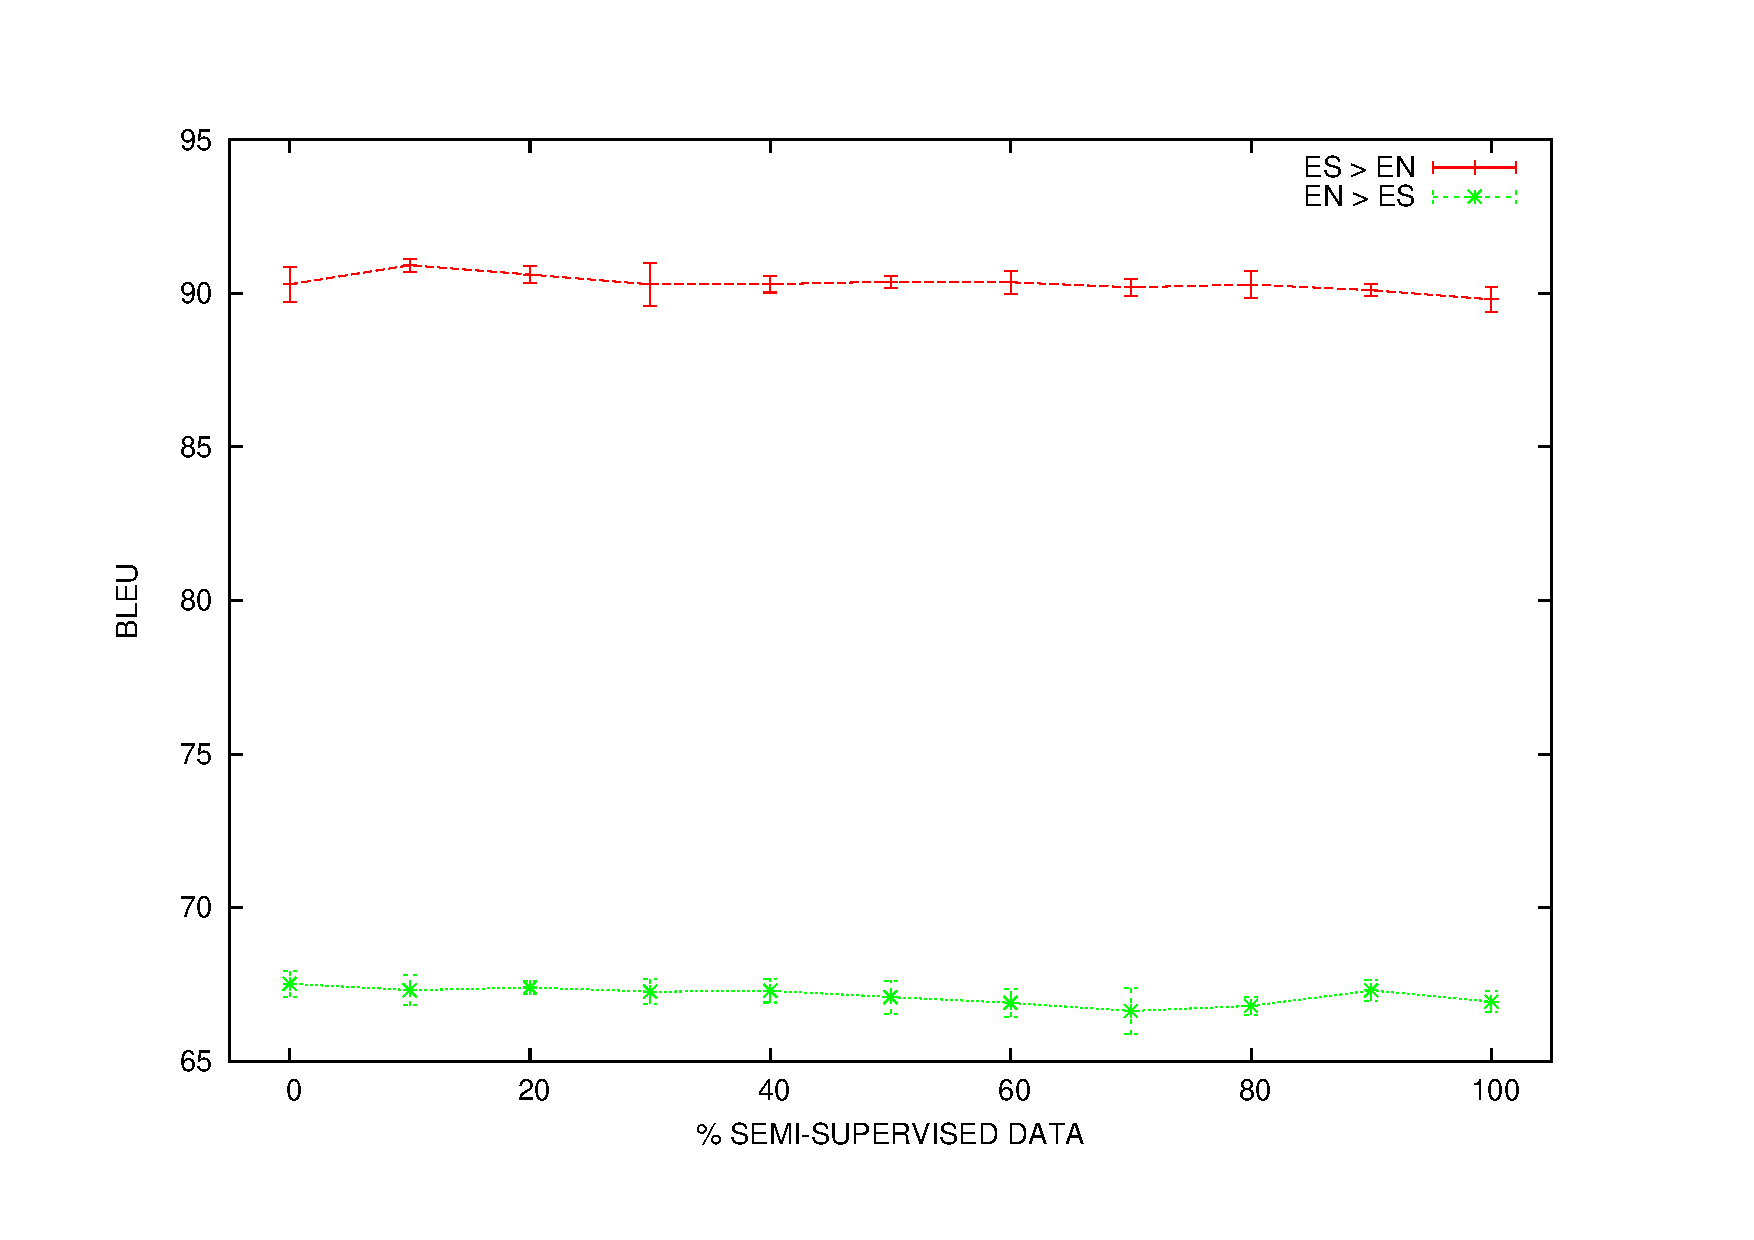
\includegraphics[width=0.8\textwidth]{UNSUPERVISED_RESULTS.pdf}
\caption{BLEU evolution when using semi-supervised data to train the models for SMT.}
\label{fig:unsupervised}
\end{figure}

As it is shown by the confidence intervals (95\%), no significant difference is observed using only supervised data or using additional semi-supervised data. The behaviour is the same translating from Spanish to English (red plot), and English to Spanish (green plot). It would be interesting to study the same effect when the amount of initial supervised data changes (for instance, using only 30\% of the original data as supervised data, or using 70\%, etc). However, these experiments were not performed.


\end{document}